\chapter{Experiment 2 - Dataset and in-Network Transformation of MNIST}
\label{chap:five}

\section{Motivation}
In order to contextualize the results of the experiments conducted on malware data, we consider the methods presented on the well-studied MNIST Database of Handwritten Digits~\cite{lecun1998mnist}.
MNIST is a benchmark in computer vision - since our baseline convolutional neural network is based on LeNet~\cite{lecun1998gradient}, we have a large body of research to compare to.
Additionally, MNIST serves as an introduction to the field of computer vision for many students and so our architectures and theories can be made more accessible in that context.
The current state of the art for MNIST achieved a 99.84 accuracy this year~\cite{byerly2020branching}.
The best results achieved in the original LeCun paper were 99.3\% accuracy; generally, accuracy greater than 97\% is considered to be good.

\section{Methodology}
In order to maintain consistency with our other findings, our methodology is the same as experiments in Chapter~\ref{chap:three}.
We leverage the hardware described in Appendix~\ref{append:one} and perform two sub-experiments.
The goal of the first part of our experiment is to best fit the data while ensuring generalization, and our goal is to optimize accuracy on the test set.
The results of this experiment are contained in Table~\ref{Tab:test}.
In the second part of our experiment, we ran the same mutual information computation as described in Section~\ref{MI computation}, and those results are displayed in Figure~\ref{fig:mnist fc infoplane} and Figure~\ref{fig:mnist conv infoplane}.

\section{Results}
In this experiment, all of our models achieve accuracy over 97\% which is broadly considered to be the benchmark accuracy for ``passing'' MNIST. 
For all these combinations of architecture and transformation, the difference between our maximum accuracy score of 99.11\% and our minimum accuracy of 97.73\% is only 1.38\%.
Comparing the convolutional models in particular, the difference between the Raw, Fourier-transformed, and Wavelet-transformed data is only 0.01\%. 

\begin{table}[h!]
\centering	
\begin{tabular}{l|ll}
\textbf{Data and Architecture}  & \textbf{Test Accuracy} & \textbf{Mean Step Time} ($\mu$s) \\\cline{1-3}
Raw, Fully-Connected NN            & 97.73\%         & 29\\
Fourier, Fully-Connected NN        & 98.12\%         & 41\\
Wavelet, Fully-Connected NN        & 97.83\%         & 30\\
\hline
Raw, Convolutional NN              & 99.11\%         & 204\\ 
Fourier, Convolutional NN          & 99.10\%         & 237\\
Wavelet, Convolutional NN          & 99.10\%         & 212\\
\hline
Raw, Fourier NN                    & 98.45\%         & 959\\
Raw, Wavelet NN                    & 98.89\%         & 1068\\ 
\end{tabular}
\caption{Neural Network Results}
\label{Tab:test}
\end{table}

\begin{figure}[h]
\begin{center}
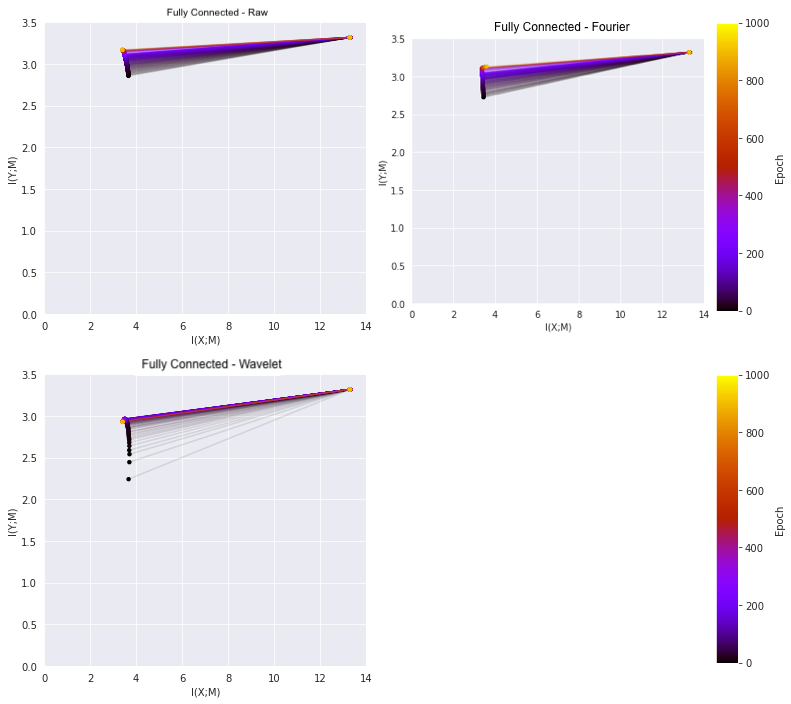
\includegraphics[width=0.8\textwidth]{mnist_fc_infoplane}
\caption{Fully-Connected Neural Network Information Plane.}
\label{fig:mnist fc infoplane}
\centering
\end{center}
\end{figure}
Figure~\ref{fig:mnist fc infoplane} was produced using the upper bound methodology from Saxe~\cite{saxe2019information}. 
We see from all three subplots in Figure ~\ref{fig:mnist fc infoplane} that over 1000 training epochs, the mutual information about the labels for the first and last layers of the neural net is quite similar for our fully-connected neural networks irrespective of the initial data.
As seen in both Shwartz-Ziv~\cite{shwartz2017opening} and Saxe~\cite{saxe2019information}, the early training epochs cause the largest increase in mutual information with respect to the labels, decreasing over training. 
We also observe a slight decrease in the amount of mutual information with respect to the data in later training epochs - which is expected as the learned representation becomes better able to map data to labels. 
The fully connected network converges to an upper bound for the output layer which is within half a bit across all three datasets - raw, Fourier-transformed, and Wavelet-transformed - within the first 500 epochs and begin to reduce their mutual information about $X$ as the network overfits the dataset.
Since we use ReLU activation functions, we do not see a ``fitting phase and compression phase'' as observed in Tishby~\cite{tishby2015deep}, who used a tanh activation, but instead a simultaneous fitting and compression as in Saxe.

\begin{figure}[h!]
\begin{center}
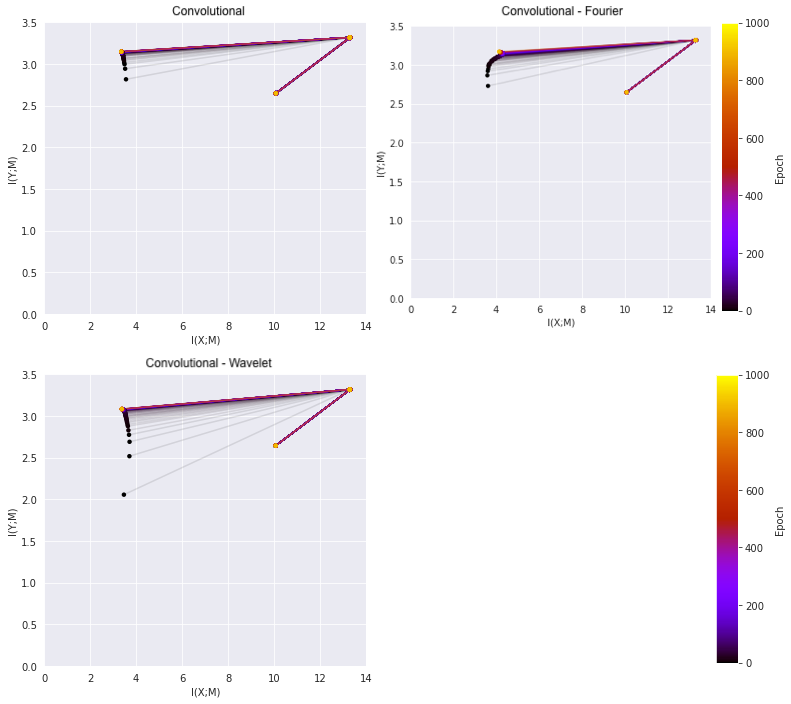
\includegraphics[width=0.8\textwidth]{mnist_conv_infoplane}
\caption{Convolutional Neural Network Information Plane}
\label{fig:mnist conv infoplane}
\centering
\end{center}
\end{figure}

We observe very similar results in Figure~\ref{fig:mnist conv infoplane} with the convolutional network, though there is some odd behavior in layer 0 in late training epochs, where mutual information in layer 0 with respect to the dataset $X$ increases and departs from our trend line.

Worth noting is that this phenomenon is consistent for our convolutional neural network across all 3 training data sets and does not appear to affect our accuracy in any negative way.
This consistency is surprising, and we discuss it in the context of our other experiments in chapter~\ref{chap:conclusion}.